%% USEFUL LINKS:
%% -------------
%%
%% - UiO LaTeX guides:          https://www.mn.uio.no/ifi/tjenester/it/hjelp/latex/
%% - Mathematics:               https://en.wikibooks.org/wiki/LaTeX/Mathematics
%% - Physics:                   https://ctan.uib.no/macros/latex/contrib/physics/physics.pdf
%% - Basics of Tikz:            https://en.wikibooks.org/wiki/LaTeX/PGF/Tikz
%% - All the colors!            https://en.wikibooks.org/wiki/LaTeX/Colors
%% - How to make tables:        https://en.wikibooks.org/wiki/LaTeX/Tables
%% - Code listing styles:       https://en.wikibooks.org/wiki/LaTeX/Source_Code_Listings
%% - \includegraphics           https://en.wikibooks.org/wiki/LaTeX/Importing_Graphics
%% - Learn more about figures:  https://en.wikibooks.org/wiki/LaTeX/Floats,_Figures_and_Captions
%% - Automagic bibliography:    https://en.wikibooks.org/wiki/LaTeX/Bibliography_Management  (this one is kinda difficult the first time)
%%
%%                              (This document is of class "revtex4-1", the REVTeX Guide explains how the class works)
%%   REVTeX Guide:              http://www.physics.csbsju.edu/370/papers/Journal_Style_Manuals/auguide4-1.pdf
%%
%% COMPILING THE .pdf FILE IN THE LINUX IN THE TERMINAL
%% ----------------------------------------------------
%%
%% [terminal]$ pdflatex report_example.tex
%%
%% Run the command twice, always.
%%
%% When using references, footnotes, etc. you should run the following chain of commands:
%%
%% [terminal]$ pdflatex report_example.tex
%% [terminal]$ bibtex report_example
%% [terminal]$ pdflatex report_example.tex
%% [terminal]$ pdflatex report_example.tex
%%
%% This series of commands can of course be gathered into a single-line command:
%% [terminal]$ pdflatex report_example.tex && bibtex report_example.aux && pdflatex report_example.tex && pdflatex report_example.tex
%%
%% ----------------------------------------------------


\documentclass[english,notitlepage,reprint,nofootinbib]{revtex4-1}  % defines the basic parameters of the document
%,biblatex

% Allows special characters (including æøå)
\usepackage[utf8]{inputenc}

%\usepackage[
%backend=biber,
%style=alphabetic,
%sorting=none
%]{biblatex}
\usepackage{physics,amssymb}  % mathematical symbols (physics imports amsmath)
\include{amsmath}
\usepackage{graphicx}         % include graphics such as plots
\usepackage{xcolor}           % set colors
\usepackage{hyperref}         % automagic cross-referencing
\usepackage{listings}         % display code
\usepackage{subfigure}        % imports a lot of cool and useful figure commands
\usepackage{float}
%\usepackage[section]{placeins}
\usepackage{algorithm}
\usepackage[noend]{algpseudocode}
\usepackage{subfigure}
\usepackage{tikz}
\usepackage{xcolor}
\usetikzlibrary{quantikz}
\usepackage{pgf}
\usepackage{enumerate}


% defines the color of hyperref objects
% Blending two colors:  blue!80!black  =  80% blue and 20% black
\hypersetup{ % this is just my personal choice, feel free to change things
    colorlinks,
    linkcolor={red!50!black},
    citecolor={blue!50!black},
    urlcolor={blue!80!black}}

\usepackage{algorithm}
\usepackage[noend]{algpseudocode}
\usepackage{algpseudocode}
\bibliographystyle{apsrev4-2}



%\addbibresource{references.bib} % Imports bib file
% ===========================================
                       % self-explanatory
\begin{document}
\title{Analyzing Covid data to discover factors associated with death}  % self-explanatory
\author{Erlend Kristensen, Mathias Mellemstuen, Magnus Selmer-Anderssen Kråkenes} % self-explanatory
\date{\today}      


\noaffiliation                            % ignore this, but keep it.

%This is how we create an abstract section.
\begin{abstract}
    In this project we analyzed Covid-19 data of people who died or did not die of Covid-19. The data set consisted of $21$ features, such as whether or not someone had diabetes. We started out by using MLP and Random forest classifiers to try to predict whether someone with Covid-19 would die or not, and found Random forest to be a better classifier for this. We also extracted the feature importance using the Random forest classifier, and found age to be the most important feature. We then looked into the chance of dying based on age, and tried to fit a linear regression model to this data with as few samples as possible, and figured we only needed about $200 000$ samples to fully predict the death rate of Covid-19. After this we compared the death rate of the general population compared to those with diabetes, and found that those with diabetes were at larger risk of dying from Covid-19 across all age groups. With this we proved that combining data analysis with machine learning can be an important tool for predicting the health risks for a new virus outbreak and see which groups are more at risk, so we know who to prioritize for vaccines and other treatment methods.
\end{abstract}
\maketitle


% ===========================================

\section{Introduction}
\label{sec:INTRODUCTION}
% Motivate the reader, the first part of the introduction always gives motivation and tries to give the overarching ideas
The Covid-19 pandemic has caused the death of at least 6.6 million people [World Health Organization (WHO) (\ref{ref: numberOfDeaths}), 2022]. Lockdowns were introduced to reduce the disease's spread, and while effective, the lockdowns have negatively impacted both the physical and mental health of the people, while also seriously hampering the economy of the world. Experts fear we now face a new wave of the disease [Folkehelseinstituttet (FHI) (\ref{ref: ukerapport_corona}), 2022], and there is a possibility that we will never truly rid ourselves of it and that it is something we will have to learn to live with. 
To prepare for such an eventuality, we want to create a tool to evaluate the major contributing factors to death due to the disease. By settling which groups are more at risk, we hope to provide improved health recommendations to the public. 
% Huskeliste: Få inn litt om status til problemet.

% What we have done 
\\
 We will utilize two different machine learning algorithms: The \textit{Multilayer Perceptron} (MLP) and \textit{Random Forest}. The two algorithms are trained with a huge covid dataset to classify the likelihood of death based on a large number of features. Once the algorithms are trained, we will analyze the models to extract the relative importance of each feature. We will then use simple regression methods to further investigate the most important contributing features. %The results will then be compared to the results of previous studies (FØR INN KILDE HER). 
 
% At the end of the introduction you should give a brief summary of the structure of the report
\\
We will introduce the necessary background and theory in section \ref{sec: METHODS}. In section \ref{sec: IMPLEMENTATION} we will explain how we have implemented the machine learning algorithms to get our results. The code itself can be accessed in section \ref{sec: CODE}. The results are presented and discussed in section \ref{sec: DISCUSSION}. Here we will also compare our results to previous studies. In section \ref{sec: CONCLUSION} we will present our conclusion and suggest further work. 

\section{THEORY AND METHODS}
\label{sec: METHODS}

%\subsection{Covid-19} % Ha denne her? kanskje bedre å diskutere dette i diskusjonen sammen med våre resultater. 
% Mention relevant studies, what have they found? Risk factors

\subsection{Data set}\label{subsec: DATA}
% Where is the data from, what does it contain, and how have we treated it?
We will use a publicly available data set (\ref{sec: Dataset}) in our investigation. The data is provided by the Mexican government, and it contains approximately one million samples, with up to 21 features. The majority of the features are categorical, most of which are in a yes/no fashion. In these cases, the positive case 'yes' is represented by the number 1, while the negative case 'no' is represented by the number 2. Only one feature, 'age', is numerical. 
% Hva gjør vi med dataen før vi bruker den?
However, many samples are lacking information on one or several features. In these cases, the lacking data is represented by a number between 97 and 99. %This missing data needs to be taken into consideration, as feeding the algorithms disproportionate feature data can cause them to attribute false feature importances.
% Classification problem

To discover which features are important in causing death, we will use the Random Forest classifier, which has a built-in method for this. A comparison of different machine learning algorithms also found that the Random Forest algorithm performed particularly well when predicting covid-19 mortality [Moulaei et al. (\ref{ref: Algorithm comparison}), 2022].

\subsection{Classifiers}
% Supervised learning
\subsubsection{Multilayer Perceptron}
MLP is a special case of feed forward neural networks where every layer is a fully connected layer as shown in this figure:

\begin{figure}[H]
    \centering
    \includegraphics[width=0.45\textwidth]{FYS-STK/Prosjekt_3/MLP_IMAGE.png}
    \caption{A representation of what an MLP classifier could look like.}
    \label{fig: 1}
\end{figure}
%\includegraphics[width=0.45\textwidth]{FYS-STK/Prosjekt_3/MLP_IMAGE.png}
%\caption{A representation of what an MLP classifier could look like.}
\\
\\
The use for MLP compared to a normal feed forward neural network is when we don't know a lot about the structure of the problem. Using fully connected layers allows us to learn the structure, rather than impose it [Alex \ref{ref:MLP kilde}]. 
For more on feed forward neural networks, have a look at our previous report on it found \href{https://github.com/erlend1202/FYS_STK4155_Prosjekt_2}{here}.

% Information moves forward through the layers
% Non-linear activation function
% Fully connected FFNN: Each node in a layer is connected to all nodes in the subsequent layer

% Activation functions: relu, sigmoid, tanh
% L2 regularization: Alpha
% Back propagation

\subsubsection{Random Forest}
The random forest classifier is built on the method we call \textit{decision trees}. A decision tree starts with a simple question and follows it up with more questions to determine a yes or no answer. In our case, this question would be "will covid kill this person?", followed by questions of whether or not this person has different diseases or complications found in our data set features. Each time a question is asked, we get two different branches, one for yes and one for no. The answers to our original question are at the very end, and are called \textit{leaf nodes}. 
\begin{figure}[H]
    \centering
    \includegraphics[width=0.45\textwidth]{FYS-STK/Prosjekt_3/DecisionTree.png}
    \caption{A representation of what a decision tree would look like, asking the question "is this person fit?".}
    \label{fig: 2}
\end{figure}
%\includegraphics[width=0.45\textwidth]{FYS-STK/Prosjekt_3/DecisionTree.png}
%\caption{A representation of what a decision tree would look like, asking the question "is this person fit?".}
\\
\\
A random forest classifier, however, uses feature randomness to create an uncorrelated forest of decision trees. So while decision trees consider all possible features, random forest selects only a subset of these for each tree, and uses all the trees in combination to find an answer [IBM \ref{ref:RandomForest Kilde}].


% Ensemble method
% Decision trees
% CART algorithm, cost function
% Bootstrapping

% Gini-index?

\subsection{Evaluation}
Since the task of classifying whether someone dies of covid or not is pretty difficult and complex, we will need to look at more than one form of performance measurement other than accuracy. We will therefore also look at \textit{F1-score}, which can be given by this formula:
\begin{align}
    F_1 = 2*\frac{precision*recall}{precision + recall} = \frac{2tp}{2tp + fp + fn}
\end{align}
where \textit{tp} is true positives, \textit{fp} is false positives, and \textit{fn} is false negatives.
% \subsection{Regression}
% Based on previous research we expect age to be a contributing factor. 
% We will use linear regression to investigate the connection between age and death
% Ordinary least squares


% Metastudie/rapport om risikofaktorer og dødelighet: https://www.fhi.no/publ/2020/Covid-19-og-risikofaktorer-for-alvorlig-sykdom-en-hurtigoversikt-andre-oppdatering/
\section{Implementation}\label{sec: IMPLEMENTATION}
We will use the built in classifiers in the \emph{Scikit-learn} library, such as the MLP classifier and forest of trees classifier (Random forest). We will have to preprocess the data to fit our models, such as changing the dates of death to simply a binary $1$ if dead or $0$ if alive. We will first use MLP and Random forest to see how well these classifiers are able to predict whether someone dies of covid or not. Then, we will extract the most important features from the Random forest classifier. We will also use sklearns linear regression and polynomial features on our data to predict the probability of dying from covid based on age and then add in other factors later. 
\\
How the different classifiers work and how to use them can be found on these links: 
\href{https://scikit-learn.org/stable/modules/generated/sklearn.neural_network.MLPClassifier.html}{MLP},
\href{https://scikit-learn.org/stable/modules/generated/sklearn.ensemble.RandomForestClassifier.html}{RandomForestClassifier},
\href{https://scikit-learn.org/stable/modules/generated/sklearn.preprocessing.PolynomialFeatures.html}{Polynomial features},
\href{https://scik,it-learn.org/stable/modules/generated/sklearn.linear_model.LinearRegression.html}{Linear regression}.
\\
\\
We will also start by looking at the \textit{bias-variance tradeoff} for our two classification methods, as well as linear regression methods for \textit{OLS},\textit{Lasso} and \textit{Ridge} regression (more on these can be found \href{https://github.com/mathiasmellemstuen/FYS-STK4155-Prosjekt-1}{here}, but it is not essential for this report). To do this we used regression with the \textit{Franke function}, which is a $2$-dimensional function (see Appendix \ref{eq:FrankeFunction}), and is often used to train networks for regression problems due to its complexity. 

\begin{figure}[H]
    \centering
    \includegraphics[width=0.45\textwidth]{FYS-STK/Prosjekt_2/Franke.png}
    \caption{Visual representation of the Franke function using $x,y \in [0,1]$.}
    \label{fig: 3}
\end{figure}
%\includegraphics[width=0.45\textwidth]{FYS-STK/Prosjekt_2/Franke.png}
%\caption{Figure 2: Visual representation of the Franke function using $x,y \in [0,1]$.}


% \subsection{Classification using Multilayer Perceptron}
% % Using premade sklearn functionalities, explain parameter choices
% % Jupyter?
% Our MLP model is created using the pre-existing '\href{https://scikit-learn.org/stable/modules/generated/sklearn.neural_network.MLPClassifier.html}{MLPClassifier}' class from the \emph{Scikit-learn} library. We utilize the adam solver, as this is what is recommended in the MLPClassifier-documentation for large datasets. The values for the alpha and momentum hyperparameters are decided by performing a grid search with values ranging from $10^{-5}$ to 10 and $10^{-6}$ to 1 respectively. This is done for all three activation functions described in (skriv om relu, sigmoid og tanh i metoder). The final architecture of the neural network is described in table \ref{table:1}.
% % Beskriv input og output layer
% \begin{table}[h!]
% \centering
% \begin{tabular}{|c|c|c|} 
%  \hline 
%  Layer & Nodes & Activation Function \\ [0.5ex] 
%  \hline
%  Input & x & x \\ \hline % Jeg ser vi bruker ulike størrelser på hidden layers i grid search og i main?
%  Hidden Layer 1 & 12 & tanh \\ \hline
%  Hidden Layer 2 & 10 & tanh \\ \hline
%  Hidden Layer 3 & 8 & tanh \\ \hline
%  Output & 1 & x \\ [1ex] \hline
% \end{tabular}
% \caption{Architecture of the MLP}
% \label{table:1}
% \end{table}

% Grid search to find the optimal hyperparameters
% Test for the three activation functions with the hyperparameters we have found
%  Tester vi for ulike størrelser på hidden layers? solver?

% I dokumentasjonen til MLPClassifier står det at momentum-parameteren kun brukes dersom solver er SGD?
% Men figurene gir jo klart utslag på endring i momentum, skjønner ikke helt hva som skjer her

% Hidden layers, nodes (architecture).

% \subsection{Classification using Random Forest}
% As we did with our MLP classifier, we use \href{https://scikit-learn.org/stable/modules/generated/sklearn.ensemble.RandomForestClassifier.html}{RandomForestClassifier} class from the \emph{Scikit-learn} library to create our Random Forest model. 
% % Random forest, fit to the split data
% % Perform prediction
% % Extract the feature importances


\section{RESULTS AND DISCUSSION}\label{sec: DISCUSSION}
Before we start analyzing the data, we want to look into the bias-variance tradeoff for our two classification models and linear regression models. This is to study the optimal balance in complexity for the models.  

\begin{figure}[H]
    \centering
    \includegraphics[width=0.45\textwidth]{FYS-STK/Prosjekt_3/OLS_BIAS.png}
    \caption{Plot of bias-variance tradeoff for OLS regression. x-axis is number of polynomials used. Made using franke function with $x,y \in [0,1]$, so $100 \times 100$ data points.}
    \label{fig: OLS_BIAS}
\end{figure}

\begin{figure}[H]
    \centering
    \includegraphics[width=0.45\textwidth]{FYS-STK/Prosjekt_3/RIDGE_BIAS.png}
    \caption{Plot of bias-variance tradeoff for Ridge regression. x-axis is number of polynomials used. Made using franke function with $x,y \in [0,1]$, so $100 \times 100$ data points.}
    \label{fig: RIDGE_BIAS}
\end{figure}

\begin{figure}[H]
    \centering
    \includegraphics[width=0.45\textwidth]{FYS-STK/Prosjekt_3/LASSO_BIAS.png}
    \caption{Plot of bias-variance tradeoff for Lasso regression. x-axis is number of polynomials used. Made using franke function with $x,y \in [0,1]$, so $100 \times 100$ data points.}
    \label{fig: LASSO_BIAS}
\end{figure}

As we can see from figures \ref{fig: OLS_BIAS}, \ref{fig: RIDGE_BIAS}, \ref{fig: LASSO_BIAS}, the optimal number of polynomials for OLS is about 6, while for Ridge and Lasso, the bias-variance tradeoff is more stable, but results in a worse MSE for the optimal solution compared to OLS.
This means that OLS might be best performing for certain scenarios, but Lasso and Ridge being more stable means they might generally be better choices.
\\
\\
We now do the same for our MLP and Random forest classifiers:

\begin{figure}[H]
    \centering
    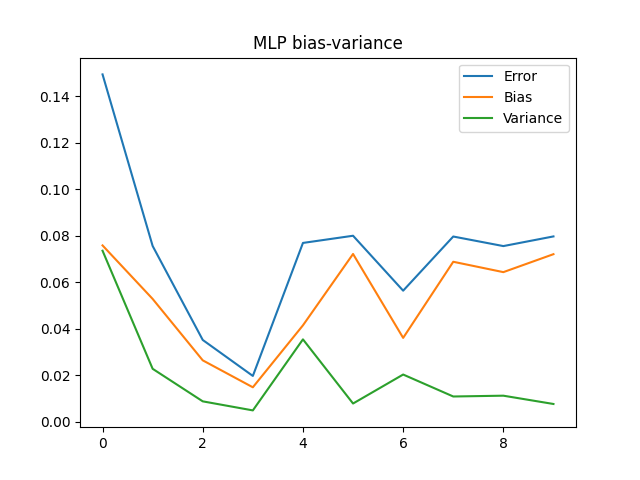
\includegraphics[width=0.45\textwidth]{FYS-STK/Prosjekt_3/MLP_bias_variance_layers.png}
    \caption{Plot of bias-variance tradeoff for MLP. x-axis is number of layers used. Made using franke function with $x,y \in [0,1]$, so $100 \times 100$ data points.}
    \label{fig: MLP_BIAS}
\end{figure}

\begin{figure}[H]
    \centering
    \includegraphics[width=0.45\textwidth]{FYS-STK/Prosjekt_3/BIAS_FOREST.png}
    \caption{Plot of bias-variance tradeoff for Random forest classifier. x-axis is minimum number of samples required to be a leaf node. Made using franke function with $x,y \in [0,1]$, so $100 \times 100$ data points.}
    \label{fig: FOREST_BIAS}
\end{figure}

As we can see in figure \ref{fig: MLP_BIAS}, the bias-variance tradeoff is around 4 layers, so we will use this moving on with our data set. For the Random forest classifier that we see in figure \ref{fig: FOREST_BIAS}, the bias stayed about the same, but the variance tradeoff was at about $25$ samples for each leaf. Keep in mind that since we use regression to test the bias-variance tradeoff, it means that we might get a different result than if we tested using our classification data set. But because it is such a complex set, we chose something that is more easily used for measuring performance. 
\\
\\
We now want to analyze the different activation functions for our MLP classifier, to see how they perform on the given data set and see which hyperparameters work best. We will use a sample size of the data, consisting of $10 000$ randomly chosen points. %We get the following heatmap plots:

\begin{figure}[H]
    \centering
    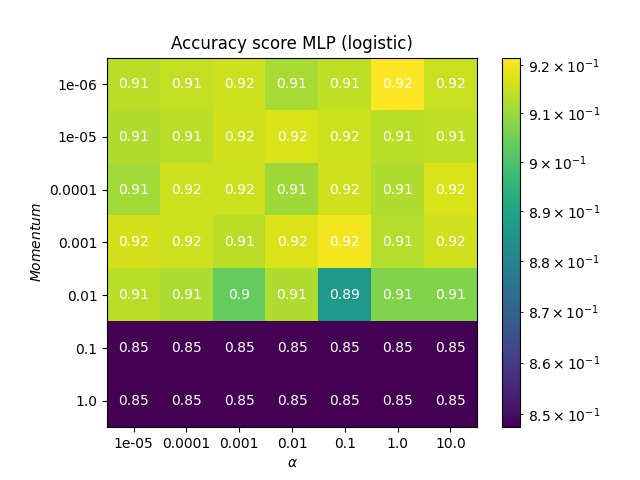
\includegraphics[width=0.45\textwidth]{FYS-STK/Prosjekt_3/Accuracy score MLP (logistic).png}
    \caption{Plot of accuracy made using layer sizes $[18,15,12,8]$ with 500 max iterations and logistic as activation function.}
    \label{fig: 4}
\end{figure}
%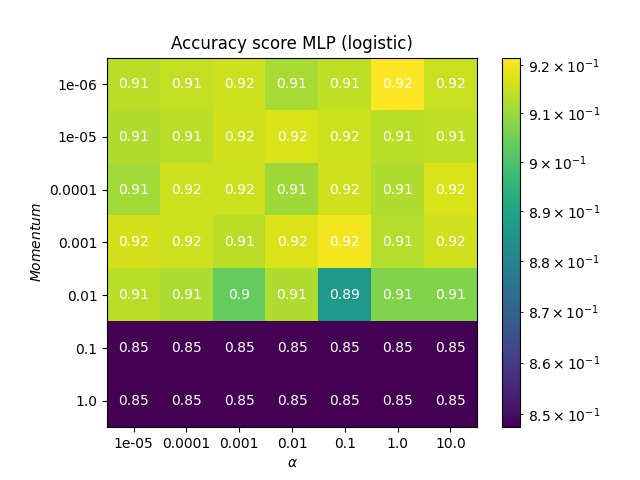
\includegraphics[width=0.45\textwidth]{FYS-STK/Prosjekt_3/Accuracy score MLP (logistic).png}
%\caption{Plot of accuracy made using layer sizes $[18,15,12,8]$ with 500 max iterations and logistic as activation function.}
\\
\begin{figure}[H]
    \centering
    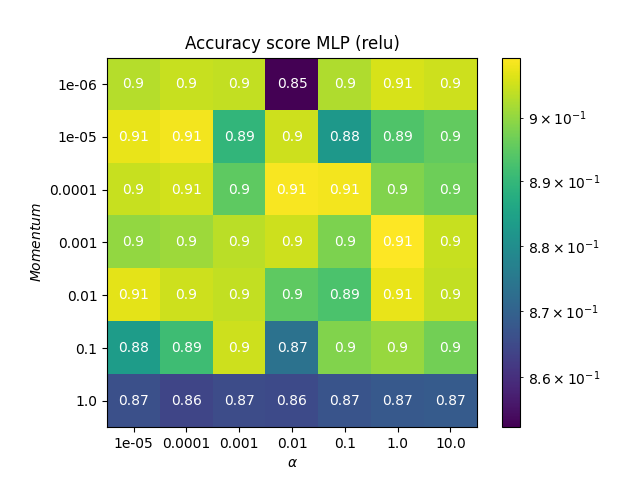
\includegraphics[width=0.45\textwidth]{FYS-STK/Prosjekt_3/Accuracy score MLP (relu).png}
    \caption{Plot of accuracy made using layer sizes $[18,15,12,8]$ with 500 max iterations and relu as activation function.}
    \label{fig: 5}
\end{figure}
%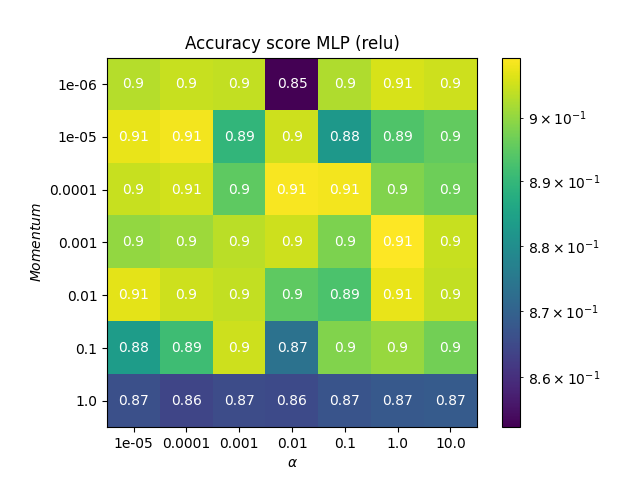
\includegraphics[width=0.45\textwidth]{FYS-STK/Prosjekt_3/Accuracy score MLP (relu).png}
%\caption{Plot of accuracy made using layer sizes $[18,15,12,8]$ with 500 max iterations and relu as activation function.}
\\
\begin{figure}[H]
    \centering
    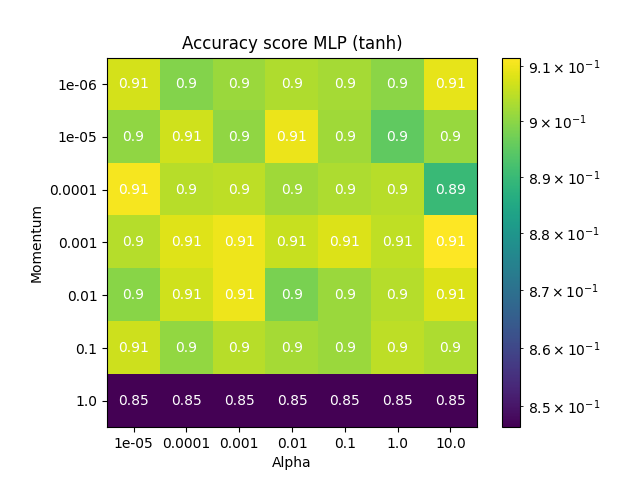
\includegraphics[width=0.45\textwidth]{FYS-STK/Prosjekt_3/Accuracy score MLP (tanh).png}
    \caption{Plot of accuracy made using layer sizes $[18,15,12,8]$ with 500 max iterations and tanh as activation function.}
    \label{fig: 6}
\end{figure}
%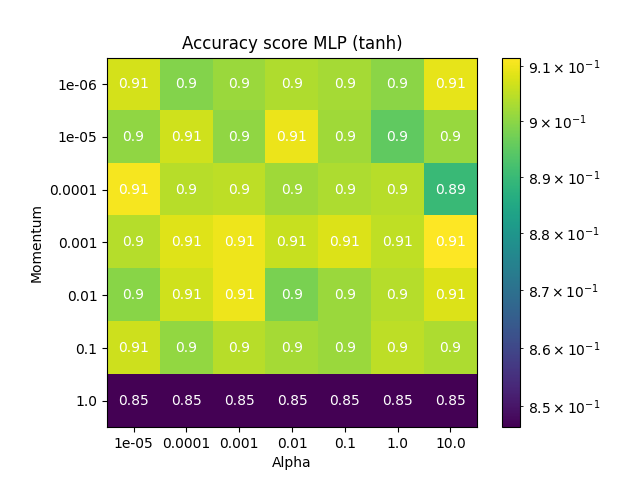
\includegraphics[width=0.45\textwidth]{FYS-STK/Prosjekt_3/Accuracy score MLP (tanh).png}
%\caption{Plot of accuracy made using layer sizes $[18,15,12,8]$ with 500 max iterations and tanh as activation function.}
\\
\\
Looking at figures \ref{fig: 4}, \ref{fig: 5}, and \ref{fig: 6}, we see that we can achieve an accuracy score of $95 \%$ for all three activation functions when using the best choice of hyperparameters. An accuracy score of around $95 \%$ is generally a good result. However, when we analyze our data, we see that the mortality rate of covid in the data set is $7 \%$. This means our data set is greatly skewed, and thus, the accuracy measurement is not enough, so we have to also analyze the F1-scores. %We do the same plots as above, just with F1-scores:
%Looking at figures \ref{fig: 4}, \ref{fig: 5}, and \ref{fig: 6}, they seem to indicate that our MLP works fine. An accuracy score of around $95 \%$ for the best choice of hyperparameters is a good result. However, when we analyze our data, we see that the mortality rate of covid in the data set is $7 \%$. This means our data set is greatly scewed, meaning an accuracy measurement is not enough, so we have to also analyze the F1-scores. We do the same plots as above, just with F1-scores:
\begin{figure}[H]
    \centering
    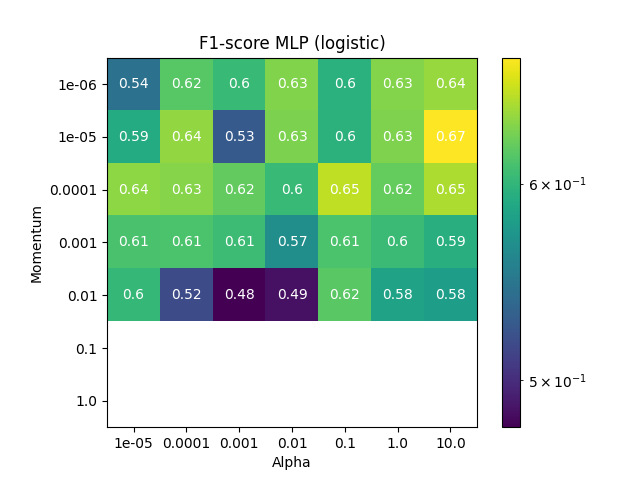
\includegraphics[width=0.45\textwidth]{FYS-STK/Prosjekt_3/F1-score MLP (logistic).png}
    \caption{Plot of F1-scores made using layer sizes $[18,15,12,8]$ with 500 max iterations and logistic as activation function.}
    \label{fig: 7}
\end{figure}
%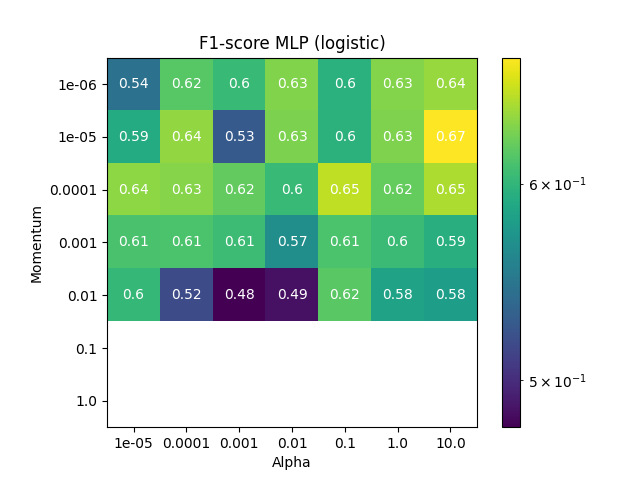
\includegraphics[width=0.45\textwidth]{FYS-STK/Prosjekt_3/F1-score MLP (logistic).png}
%\caption{Plot of F1-scores made using layer sizes $[18,15,12,8]$ with 500 max iterations and logistic as activation function.}
\\
\begin{figure}[H]
    \centering
    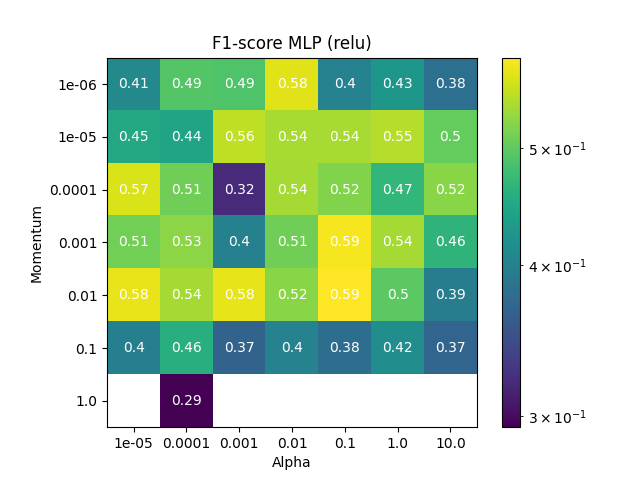
\includegraphics[width=0.45\textwidth]{FYS-STK/Prosjekt_3/F1-score MLP (relu).png}
    \caption{Plot of F1-scores made using layer sizes $[18,15,12,8]$ with 500 max iterations and relu as activation function.}
    \label{fig: 8}
\end{figure}
%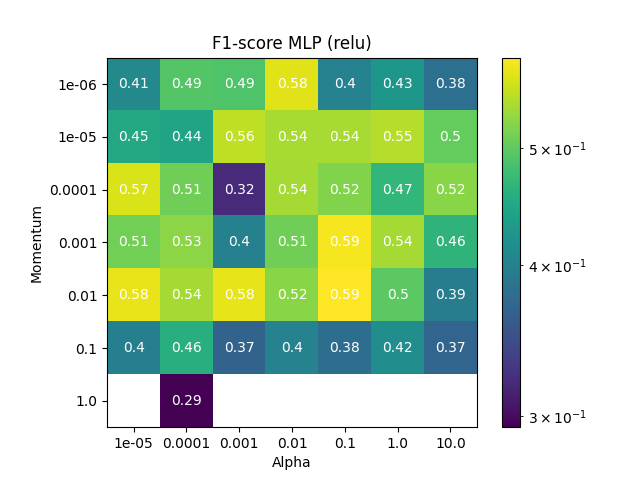
\includegraphics[width=0.45\textwidth]{FYS-STK/Prosjekt_3/F1-score MLP (relu).png}
%\caption{Plot of F1-scores made using layer sizes $[18,15,12,8]$ with 500 max iterations and relu as activation function.}
\\
\begin{figure}[H]
    \centering
    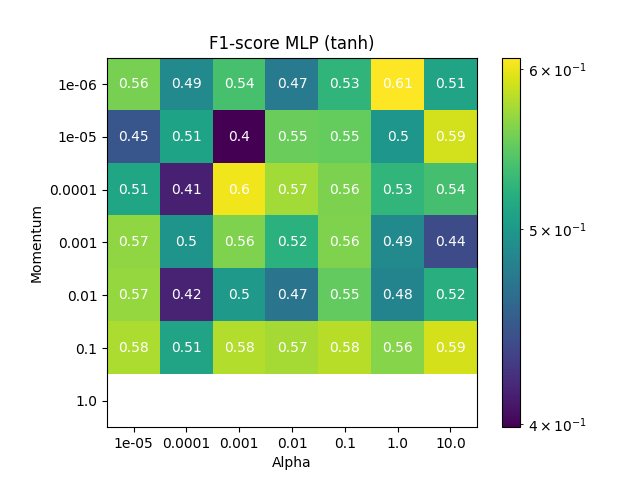
\includegraphics[width=0.45\textwidth]{FYS-STK/Prosjekt_3/F1-score MLP (tanh).png}
    \caption{Plot of F1-scores made using layer sizes $[18,15,12,8]$ with 500 max iterations and tanh as activation function.}
    \label{fig: 9}
\end{figure}
%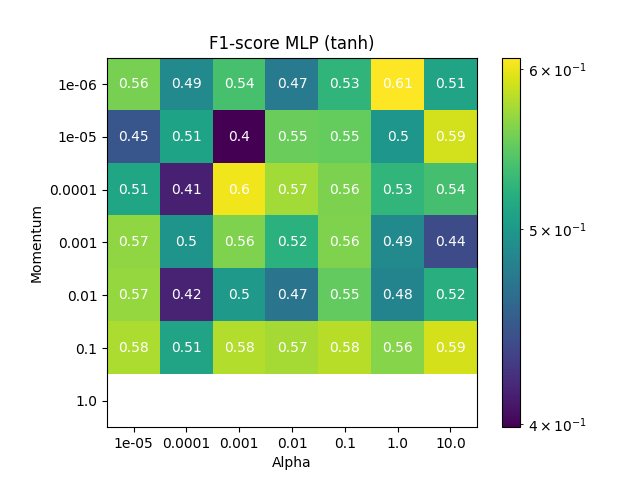
\includegraphics[width=0.45\textwidth]{FYS-STK/Prosjekt_3/F1-score MLP (tanh).png}
%\caption{Plot of F1-scores made using layer sizes $[18,15,12,8]$ with 500 max iterations and tanh as activation function.}
\\
\\
To get a good indication of which activation function performs best, we plot F1-score using the best overall hyper-parameters, with varying sample sizes: % Hva er de beste hyperparameterne egentlig? Jeg ser vi bruker alpha = 0.01 og momentum = 0.001, men det er jo ulikt for de ulike funksjonene

\begin{figure}[H]
    \centering
    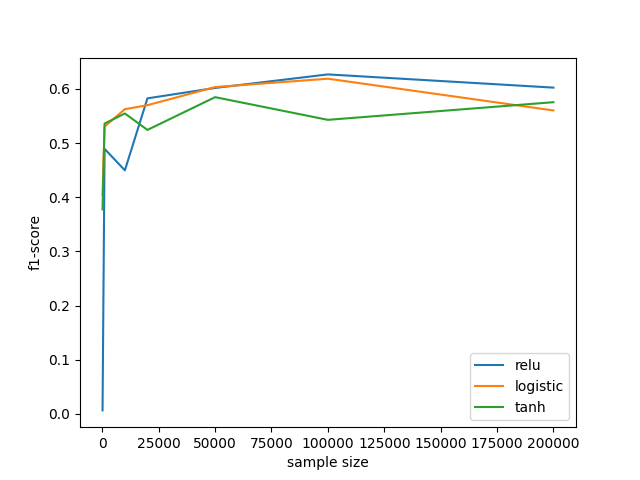
\includegraphics[width=0.45\textwidth]{FYS-STK/Prosjekt_3/f1_scores.png}
    \caption{Plot of F1-scores for tanh, relu and logistic activation function made using layer sizes $[18,15,12,8]$ with 500 max iterations, $\alpha = 0.01$ and momentum $= 0.001$.}
    \label{fig: 10}
\end{figure}
%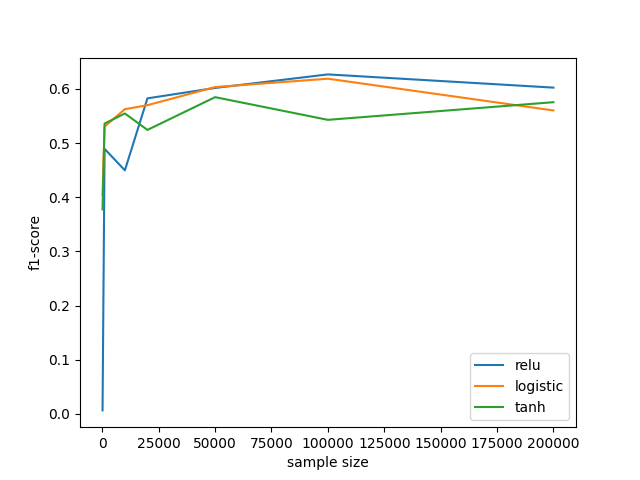
\includegraphics[width=0.45\textwidth]{FYS-STK/Prosjekt_3/f1_scores.png}
%\caption{Plot of F1-scores for tanh, relu and logistic activation function made using layer sizes $[18,15,12,8]$ with 500 max iterations, $\alpha = 0.01$ and momentum $= 0.001$.}
\\
By analyzing the heatmaps shown in figures \ref{fig: 7}, \ref{fig: 8}, and \ref{fig: 9}, it seems as if the logistic function is the best activation function for a very low sample size, as the heatmaps were calculated using a sample size of $10 000$. However, when we increase the sample size, as shown in figure \ref{fig: 10}, the relu model matches the performance of the logistic model relatively quickly. With sample sizes between $25 000$ and $100 000$, these two models perform evenly, but with sample sizes higher than this, the relu model seems to be the best choice. The tanh model is generally underperforming at all sample sizes, but while the relu and logistic models are on negative trends for sample sizes larger than $100 000$, the tanh model is on a positive trend. Thus, there is a possibility that the tanh model is a good choice for sample sizes larger than what we have tested. 
%Here, we see tanh is the best activation function for a very low sample size, as we saw with our heatmap plots using sample size 10000. However, increasing the sample size enough seems to indicate that tanh underperforms and that relu and logistic are the best options
\\
\\
 The F1-scores, which at most reach 0.67, indicate that our MLP classifier is not perfect for predicting whether someone dies of covid or not. However, as stated above in \ref{subsec: DATA}, the data set consists of $21$ features, not all as relevant as the others. It is also difficult to precisely predict someone's death with "only" $21$ features, seeing as there is no sure way of telling if someone will die from covid or not. So an F1-score of over $0.60$ is actually pretty decent in this case. 
 %This is also very similar to the result achieved by Nizri & Indik, who created an MLP on the same data set with an F1-score of 0.66 and an overall accuracy of 0.85 [Nizri & Indik, 2022] Kanskje en dum kilde, dropper denne tenker jeg
 %% huskeliste: nevne feilkilder? ingen data om covid-type eller vaksinasjonsstatus
\\
\\
We will now look at similar plots for our forest of trees classification method and see if this performs better on the given data set.

\begin{figure}[H]
    \centering
    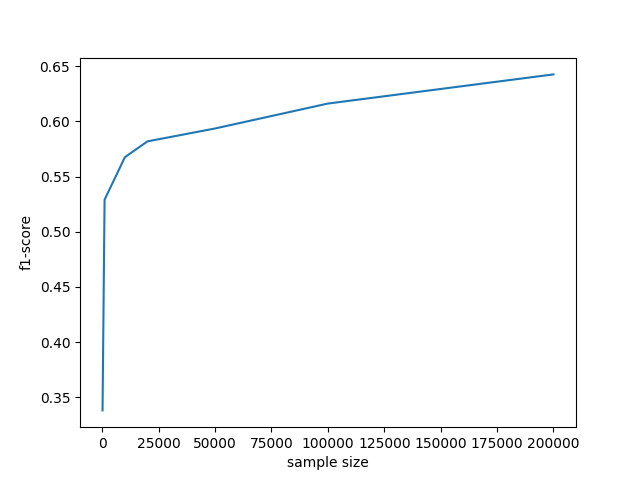
\includegraphics[width=0.45\textwidth]{FYS-STK/Prosjekt_3/f1_score_forest.png}
    \caption{Plot of F1-scores for different sample sizes for forest of trees method using scikit learns RandomForestClassifier.}
    \label{fig: 11}
\end{figure}
%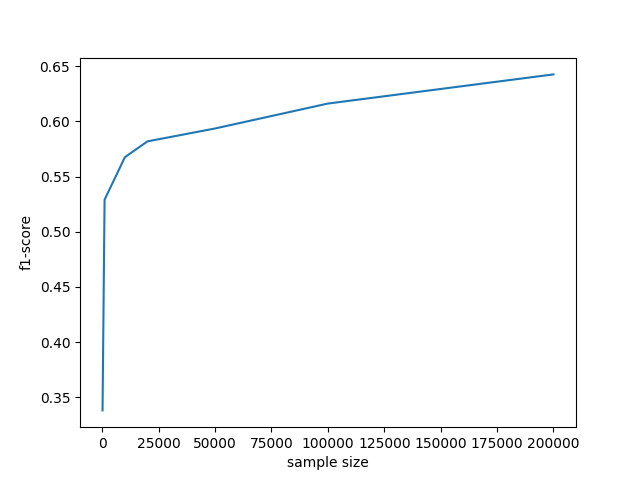
\includegraphics[width=0.45\textwidth]{FYS-STK/Prosjekt_3/f1_score_forest.png}
%\caption{Plot of F1-scores for different sample sizes for forest of trees method using scikit learns RandomForestClassifier.}
\\
\\
If we compare figure \ref{fig: 10} and \ref{fig: 11}, we see that the forest of trees has a slightly better outcome on the F1-scores than our MLP classifier. Also, in contrast to our MLP, it does not seem that forest of trees hits a max F1-score anytime during the plot. We tested this further using the whole data set, which resulted in a F1-score of $0.82$, so it seems forest of trees does a better job at classifying using the whole data set compared to MLP. This is in accordance with the previously mentioned results achieved by Moulaei et al. [Moulaei et al. (\ref{ref: Algorithm comparison}), 2022]. % Referere på nytt? Eller referere til seksjonen i teksten vår der vi sist nevnte den, noe a la: This is in accordance with the results achieved by Moulaei et al. mentioned in section \ref{subsec: DATA}
\\
\\
With forest of trees, we can extract and see which features the classifier found to be most relevant:
\begin{figure}[H]
    \centering
    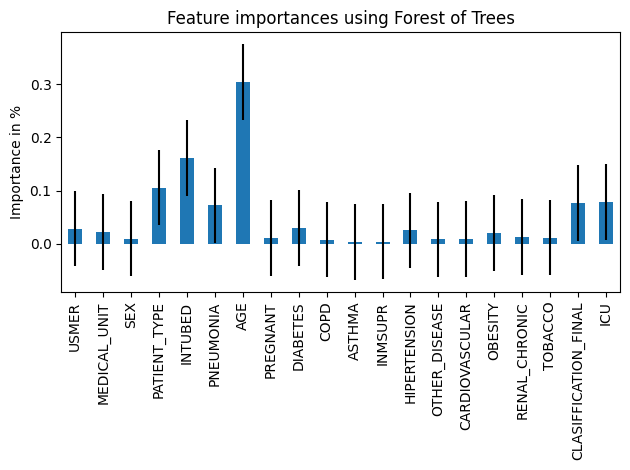
\includegraphics[width=0.45\textwidth]{FYS-STK/Prosjekt_3/Feature_importance.png}
    \caption{Plot of feature importance for forest of trees method using scikit learns RandomForestClassifier.}
    \label{fig: 12}
\end{figure}
%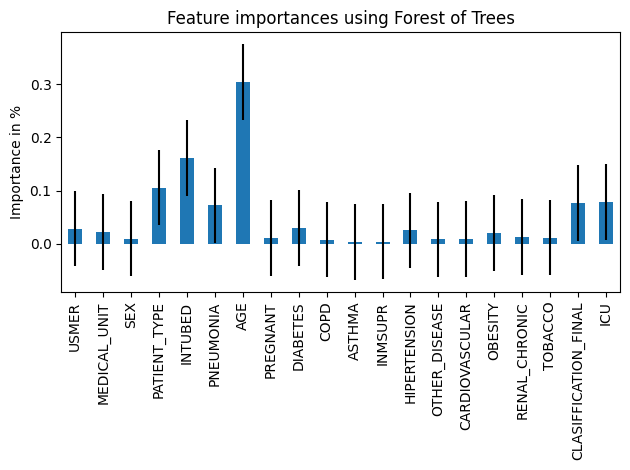
\includegraphics[width=0.45\textwidth]{FYS-STK/Prosjekt_3/Feature_importance.png}
%\caption{Plot of feature importance for forest of trees method using scikit learns RandomForestClassifier.}
\\
\\

% Rapport vi kan sammenligne med: https://www.ncbi.nlm.nih.gov/pmc/articles/PMC8485986/
% https://bmcmedinformdecismak.biomedcentral.com/articles/10.1186/s12911-021-01742-0/tables/4
% Skal vi vise til feature labels, altså (INTUBED) eller skal vi droppe det? Det er og en mulighet å lage en tabell i appendix med feature-forklaringer som vi refererer til
In figure \ref{fig: 12}, we see that two features are dominant, age and whether or not a person was connected to a ventilator (INTUBED). Less significant, but still important features include whether a person was hospitalized or not (PATIENT$\_$TYPE), whether a person was admitted to the intensive care unit or not (ICU), and whether or not a person had pneumonia at the time the sample was taken. None of these results are, by themselves, unexpected. People who need to be admitted to the hospital, the ICU, or a ventilator are already quite sick, and are thus more likely to die than the general case. What is interesting, however, is just how dominant the age factor is, dwarfing features such as diabetes, obesity, cardiovascular diseases, and immunosuppression (IMMSUPR), all of which are risk factors for covid-19 [FHI (\ref{ref: FHI risikogrupper 2}), 2022]. This goes against what was found by Moulaei et al, who reported a higher degree of importance for ICU admission than for age, and a much closer degree of importance between the age, diabetes, hypertension, and cardiovascular disease features [Moulaei et al. (\ref{ref: Algorithm comparison}), 2022]. However, this difference in results is likely caused by vastly different sample sizes, as Moulaei et al. had only $1500$ samples to work with. Either way, there is an agreement that age is a feature of high importance, which is also supported by other research [Flodgren et al (\ref{ref: FHI risikofaktorer}), 2020]. We will therefore further analyze this feature. We start by making a figure showing the total amount of deaths, and a figure showing the probability of death given age.
%we see that age is the most important feature for our predictions, even above ICU. Age as a factor is in accordance with previous research [Flodgren et al (\ref{ref: FHI risikofaktorer}), 2020]. 

\begin{figure}[H]
    \centering
    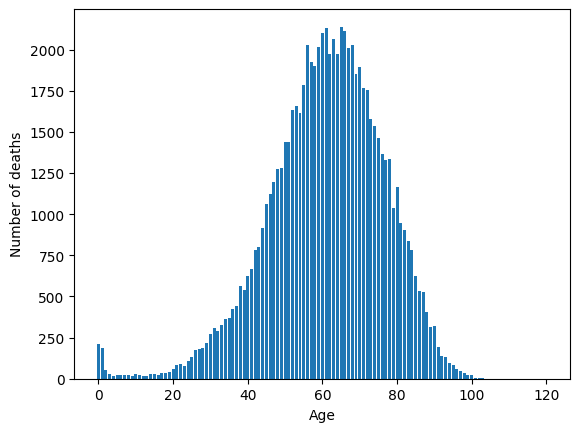
\includegraphics[width=0.45\textwidth]{FYS-STK/Prosjekt_3/number_of_deaths.png}
    \caption{Plot showing the total number of deaths at all ages.}
    \label{fig: 13}
\end{figure}
%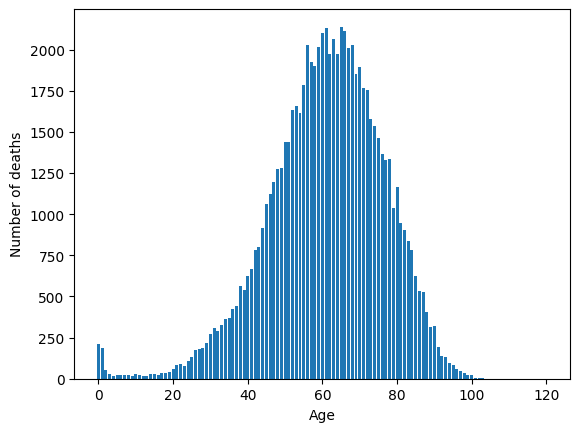
\includegraphics[width=0.45\textwidth]{FYS-STK/Prosjekt_3/number_of_deaths.png}
%\caption{Plot of total number of deaths for every age.}

\begin{figure}[H]
    \centering
    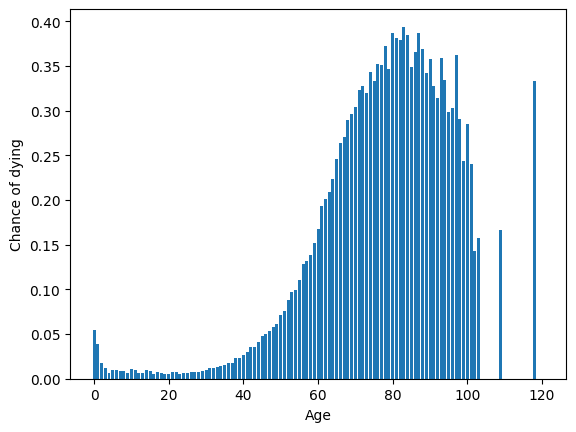
\includegraphics[width=0.45\textwidth]{FYS-STK/Prosjekt_3/chance_of_dying.png}
    \caption{Plot showing the probability of death given age.}
    \label{fig: 14}
\end{figure}
%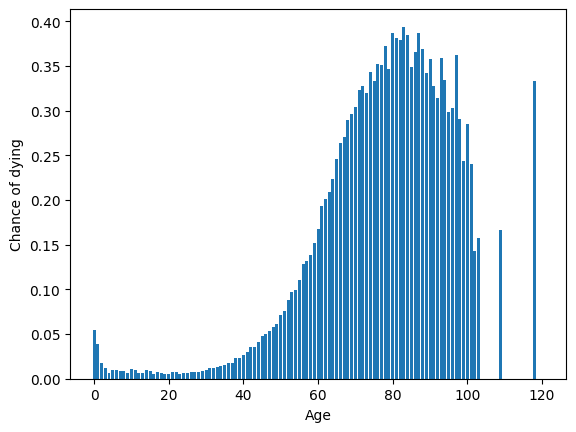
\includegraphics[width=0.45\textwidth]{FYS-STK/Prosjekt_3/chance_of_dying.png}
%\caption{Plot of chance of dying (where 1 is 100 \%) for every age.}
\\
\\
In figure \ref{fig: 14}, we see that the probability of dying is almost $40 \%$ around age 80. The reason for such a high probability could be that most of the cases reported in this data set are for those who got serious symptoms, and not just those with mild or non-existing symptoms. However, the data set still shows that even though most deaths are centered around age groups of $60$, as shown in figure \ref{fig: 13}, the probability of dying is about twice as high for those around $80$ years old. The data also shows how around age $40$, the death rate starts to exponentially increase, which means those above $40$ are at a higher risk than the rest of the population. 
% There are a few spikes in figures 14 and 15. These are very likely errors in the model, as from figure 13 we see that there are no cases of death at these ages. 
\\
This analysis gives us a great indication as to how much risk there is behind covid, and which age groups to focus on. To further study this, we will use linear regression models to see how few samples we could have and still find a probability curve good enough to predict the death rate of covid.
\begin{figure}[H]
    \centering
    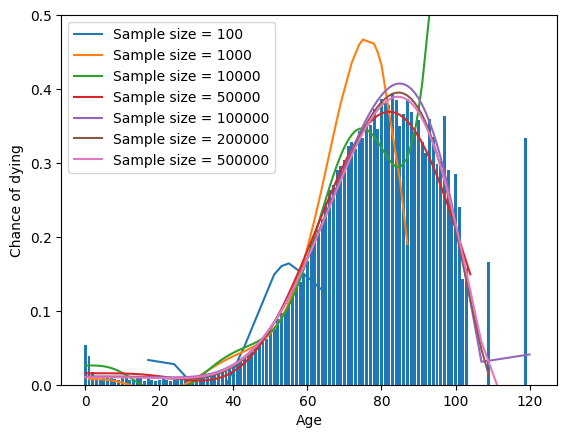
\includegraphics[width=0.45\textwidth]{FYS-STK/Prosjekt_3/chance_of_dying_differentSamples.png}
    \caption{Plot showing the probability of death for all ages using linear regression for multiple sample sizes. The samples were random as to make it as realistic as possible.}
    \label{fig: 15}
\end{figure}
%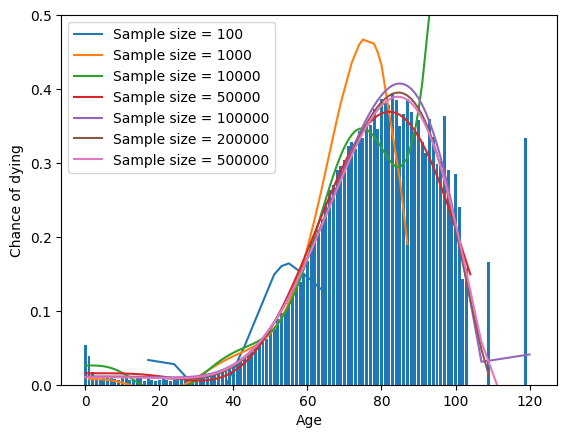
\includegraphics[width=0.45\textwidth]{FYS-STK/Prosjekt_3/chance_of_dying_differentSamples.png}
%\caption{Plot of chance of dying (where 1 is 100 \%) for every age using linear regression for multiple sample sizes. The samples were random as to make it as realistic as possible.}
\\
\\
As we see in figure \ref{fig: 15}, the plots start to really improve and fit the data set at around $50 000$ samples. To further investigate, we plot the mean squared error (MSE) using bootstrapping. 

\begin{figure}[H]
    \centering
    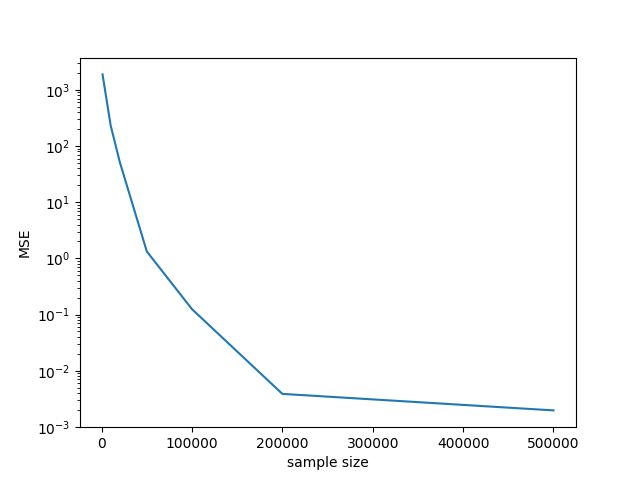
\includegraphics[width=0.45\textwidth]{FYS-STK/Prosjekt_3/MSE_Chance_dying_bootstrap_FULLDATA.png}
    \caption{Plot of MSE for our linear regression model using different random samples of different sample sizes.}
    \label{fig: 16}
\end{figure}
%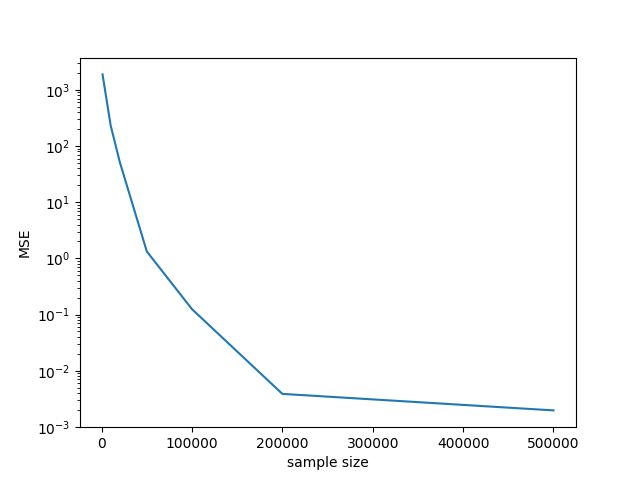
\includegraphics[width=0.45\textwidth]{FYS-STK/Prosjekt_3/MSE_Chance_dying_bootstrap_FULLDATA.png}
%\caption{Plot of MSE for our linear regression model using different random samples of different sample sizes.}
\\
\\
In figure \ref{fig: 16} we see that at about $200 000$ samples, our model is able to fit the data set more than well enough. This shows us that even though the data set consists of $1 000 000$ different cases, we only need about $200 000$ to be able to accurately predict the death rate of covid based on age. For future viruses, this would be very useful to predict how dangerous the virus is, and also which age groups should be considered a risk group.
\\
After looking into the death rate based on age, we want to combine this to examine how an underlying condition contributes to the overall death rate. Specifically, we will look at diabetes as, while not being a disease of the lungs, it is still classified as a risk group. Also, if we look at figure \ref{fig: 12}, we see that diabetes has a higher importance than asthma, which is a respiratory disease, in our random forest model. Therefore, we made a plot of the death rate based on age for those with diabetes, and compared it to the overall death rate based on age:
%Now that we have looked into the death rate based on age, we want to combine this to see how an underlying condition contributes to the overall death rate. We chose to look at diabetes, as it is a disease classified as a risk group from covid, but not a disease that affects the lungs such as asthma, so it would be interesting to see how it affects covid. Also, when we looked at figure \ref{fig: 12}, showing feature importance, diabetes was above asthma, so it would be interesting to see exactly why that is. Therefore, we made a plot of the death rate based on age for those with diabetes, and compared it to the overall death rate based on age:
\begin{figure}[H]
    \centering
    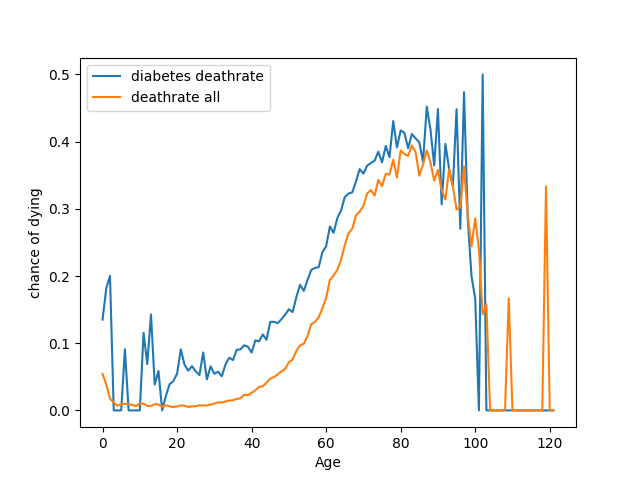
\includegraphics[width=0.45\textwidth]{FYS-STK/Prosjekt_3/death_rate_diabetes_vs_all.png}
    \caption{Plot of chance of dying (where 1 is 100 \%) for every age, comparing those with diabetes to the general population.}
    \label{fig: 17}
\end{figure}
%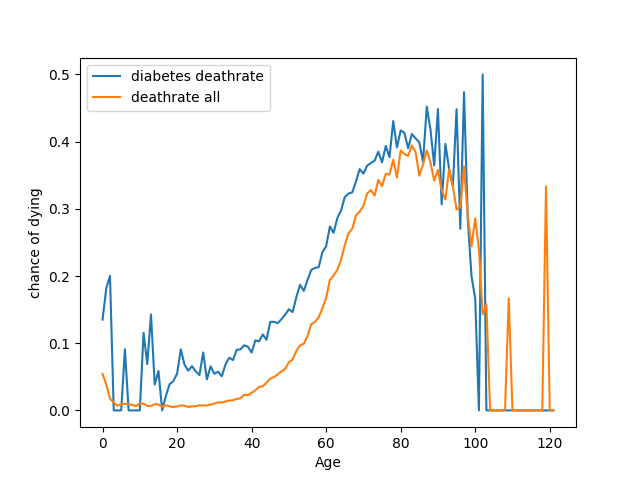
\includegraphics[width=0.45\textwidth]{FYS-STK/Prosjekt_3/death_rate_diabetes_vs_all.png}
%\caption{Plot of chance of dying (where 1 is 100 \%) for every age, comparing those with diabetes to the general population.}
\\
\\
In figure \ref{fig: 17}, we see that the curve for diabetes cases follows a very similar trend to that of the general population, but is generally a few percentage points higher. The distance between the two curves also seems to decrease somewhat as age increases. This indicates to us that people with diabetes generally are at a higher risk from covid than those without, but that diabetes is a more serious risk factor for younger age groups. % Nevne figur 12 igjen? Sammenligne hvor tydelig diabetes ser ut til å påvirke i fig 17 mot hvor liten effekt det ser ut til å ha i fig 12?
% In figure \ref{fig: 17}, we can see the curve for those with diabetes is almost identical to those without, just that it is a few percentage points above.

\section{CONCLUSION}\label{sec: CONCLUSION}
We have now tested how well classifiers such as MLP and Random forest perform when predicting whether or not a person dies of covid or not. This proved to be not as effective, seeing as covid is a disease, meaning there is likely more behind whether or not a person dies than what can be represented by the $21$ features we used. However, the models were able to produce somewhat decent results, and by using feature importance from Random forest, we were able to see more in-depth which factors play a bigger role in the disease. We analyzed the death rate based on age and found out that we only need about $200 000$ cases (samples) to be able to predict the death rate of covid well. Also adding in the death rate of those with diabetes gave us an indication that those with diabetes were indeed more at risk than the rest of the population. Using the information we gathered from this report could prove to be useful in future virus outbreaks to give us an early indication of how dangerous the virus is and who is more at risk and should be prioritized for vaccines etc. For future work, we could go more in-depth on the death rate of multiple factors and not just age and diabetes which would give us even more information on the disease. 


\section{CODE}\label{sec: CODE}
The code used in this project can be found in \href{https://github.com/mathiasmellemstuen/FYS_STK4155_Prosjekt_3}{this} Github repository.

\section{REFERENCES}\label{sec: REF}
Alex 
\href{https://boostedml.com/2020/04/feedforward-neural-networks-and-multilayer-perceptrons.html}{Feedforward Neural Networks and Multilayer Perceptrons}, (BOOSTEDML, 2020).\label{ref:MLP kilde}
\\
Flodgren et al. \href{https://www.fhi.no/globalassets/dokumenterfiler/rapporter/2020/covid-19-and-risk-factors-for-severe-disease-2nd-update-report-2020.pdf}{COVID-19 and risk factors for severe disease - a rapid review, 2nd update}, (FHI, 2020). \label{ref: FHI risikofaktorer}
\\
Folkehelseinstituttet \href{https://www.fhi.no/nettpub/coronavirus/befolkningen/risikogrupper/}{Råd og informasjon til risikogrupper og pårørende}, (FHI, 2022). \label{ref: FHI risikogrupper 2}
\\
Folkehelseinstituttet \href{https://www.fhi.no/contentassets/8a971e7b0a3c4a06bdbf381ab52e6157/vedlegg/2022/ukerapport-uke-49-05.12--11.12.22.pdf}{Covid-19, influensa og andre luftveisinfeksjoner: Rapport - uke 49}, (FHI, 2022). \label{ref: ukerapport_corona}
\\
IBM 
\href{https://www.ibm.com/cloud/learn/random-forest}{Feedforward Neural Networks and Multilayer Perceptrons}, (IBM, 2020).\label{ref:RandomForest Kilde}
\\
Moulaei, K et al. \href{https://bmcmedinformdecismak.biomedcentral.com/articles/10.1186/s12911-021-01742-0}{Comparing machine learning algorithms for predicting COVID-19 mortality}, (BMC Medical Informatics and Decision Making, 2022). \label{ref: Algorithm comparison}
\\
World Health Organization \href{https://covid19.who.int/}{WHO Coronavirus (COVID-19) Dashboard}. Accessed 28. November 2022. \label{ref: numberOfDeaths}

% Rapport vi kan sammenligne med: https://www.ncbi.nlm.nih.gov/pmc/articles/PMC8485986/

% Rapport som sammenligner ulike typer maskinlæringsalgoritmers evne til å predikere død/alvorlighet av corona: https://bmcmedinformdecismak.biomedcentral.com/articles/10.1186/s12911-021-01742-0
% De fant at random forest gjorde det spesielt bra, tenker å bruke denne til å begrunne hvorfor vi bruker RF

% xgboost på samme data som vi kan sammenligne med, med fokus på feature importance: https://www.kaggle.com/code/baturalpsert/covid19-xgboost-eda

% Om risikofaktorer: https://www.fhi.no/globalassets/dokumenterfiler/rapporter/2020/covid-19-and-risk-factors-for-severe-disease-2nd-update-report-2020.pdf
% Sammenheng mellom fedme og respirator: https://onlinelibrary.wiley.com/doi/10.1002/oby.22831

\appendix
\section{Dataset} \label{sec: Dataset}
The dataset was downloaded from: \href{https://www.kaggle.com/datasets/meirnizri/covid19-dataset}{Covid-19 Dataset}
% Vet ikke hvor eller hvordan man skal referere til dataset

\section{Numerical Notation}\label{sec:NOTATION}
\caption{Franke function:}
\label{eq:FrankeFunction}
\begin{align*}
    f(x,y) &= \frac{3}{4} exp \left( \frac{(9x -2)^2}{4} - \frac{(9y -2)^2}{4}  \right) \\
    &+  \frac{3}{4} exp \left( -\frac{(9x + 1)^2}{49} - \frac{(9y + 1)}{10} \right) \\
    &+ \frac{1}{2} exp \left( -\frac{(9x -7)^2}{4} - \frac{(9y - 3)^2}{4} \right) \\
    &- \frac{1}{5} exp \left( - (9x - 4)^2 - (9y - 7)^2 \right)
\end{align*}

\end{document}